\section{Experiments}
\subsection{Experimental Setup}
I verify the proposed PINN methods on generated dataset, and FDTD methods with hybrid and pure MPI strategies
on the server with two Intel (R) Xeon (R) Platinum 9242 CPU nodes (96 cores per node) and $4$ NUMA nodes per node.
While the dataset is using \texttt{std::m19937} STL random device with given seed $42$ \cite{STL:RANDOM_SEED}.
The PINN models I mentioned are trained using train-from-scratch strategy, and maximin number of training times is $1'000'000$ epochs.
In the setting of learning rate and optimizer, I chose to use Adam with constant learning speed $10^{-3}$.
The details of PDEs are determined in previous section \ref{SEC:Specific_Form}.  
For more settings, please refer to Appendix.

\subsection{Comparison on single node}

% Table 
% lists the results 

% \begin{table}
%   \caption{Strong Scaling on Single Node of 2D Heat Equation}
%   \label{}
%   \begin{minipage}{\columnwidth}
%     \begin{center}
%       \begin{tabular}{lcccccc}
%         \toprule
%         Scale & $1024^2$ & $2048^2$ & $4096^2$  & $8192^2$  & $16384^2$ & $32768^2$\\
%         \midrule
%         2     & 1        & 1        &   1       & 1         & 1         & 1 \\
%         4     & 1        & 1        &   1       & 1         & 1         & 1 \\
%         8     & 1        & 1        &   1       & 1         & 1         & 1 \\
%         16     & 1        & 1        &   1       & 1         & 1         & 1 \\
%         32     & 1        & 1        &   1       & 1         & 1         & 1 \\
%         48     & 1        & 1        &   1       & 1         & 1         & 1 \\
%         64     & 1        & 1        &   1       & 1         & 1         & 1 \\
%         96     & 1        & 1        &   1       & 1         & 1         & 1 \\
%         \bottomrule
%       \end{tabular}
%     \end{center}
%     % \bigskip
%     % \footnotesize\emph{Source:} This is source 
%   \end{minipage}
% \end{table}


\begin{figure}[htbp]
  \centering
  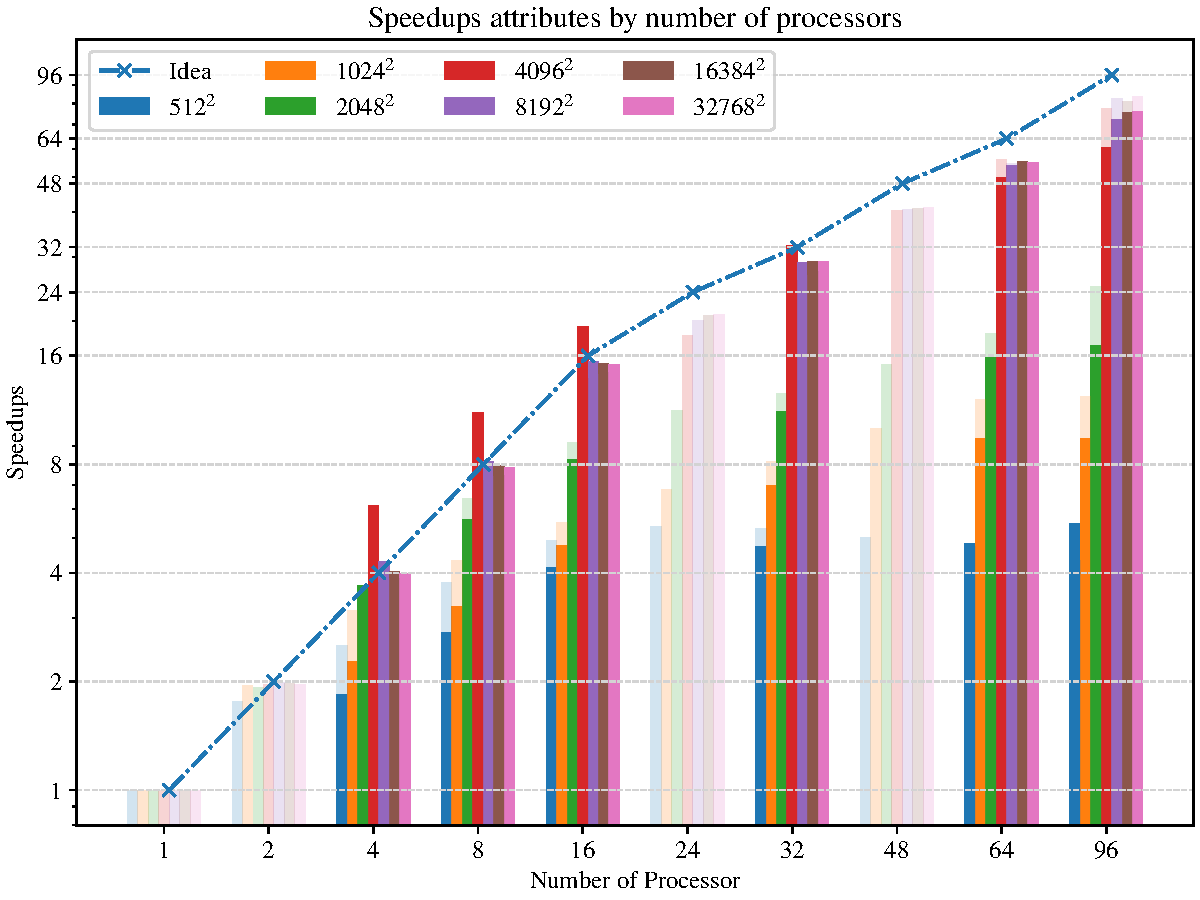
\includegraphics[width=0.8\textwidth]{figure/test_plot.pdf}
  \caption{<caption>}
  \label{<label>}
\end{figure}






\subsection{Comparison}
\subsection{Comparison}

% \subsection{Finite Difference Methods}
% \subsubsection{Pure Message Passing Parallel}
% \subsubsection{Hybrid Parallel}


% \subsection{Physics Informed Neural Networks}
% \subsubsection{CUDA parallel}
% \subsubsection{Hybrid Parallel}


\subsection{Visualization}